\section{Results on astronomical surveys}

We evaluate StarNet on two distinct surveys. First, we catalog an SDSS image of the Messier 2 (M2) globular cluster. 
We evaluate the catalog quality by validating against data collected from 
the Hubble Space telescope, which we use as a ground truth. 

Then, we run StarNet on a high-resolution DECam image of the galactic plane of the Milky Way. 
We demonstrate the ability of StarNet to scale to larger astronomical surveys.

\subsection{Results on the M2 globular cluster}
\label{sec:results_on_m2}

\begin{figure}[tb]
    \centering
    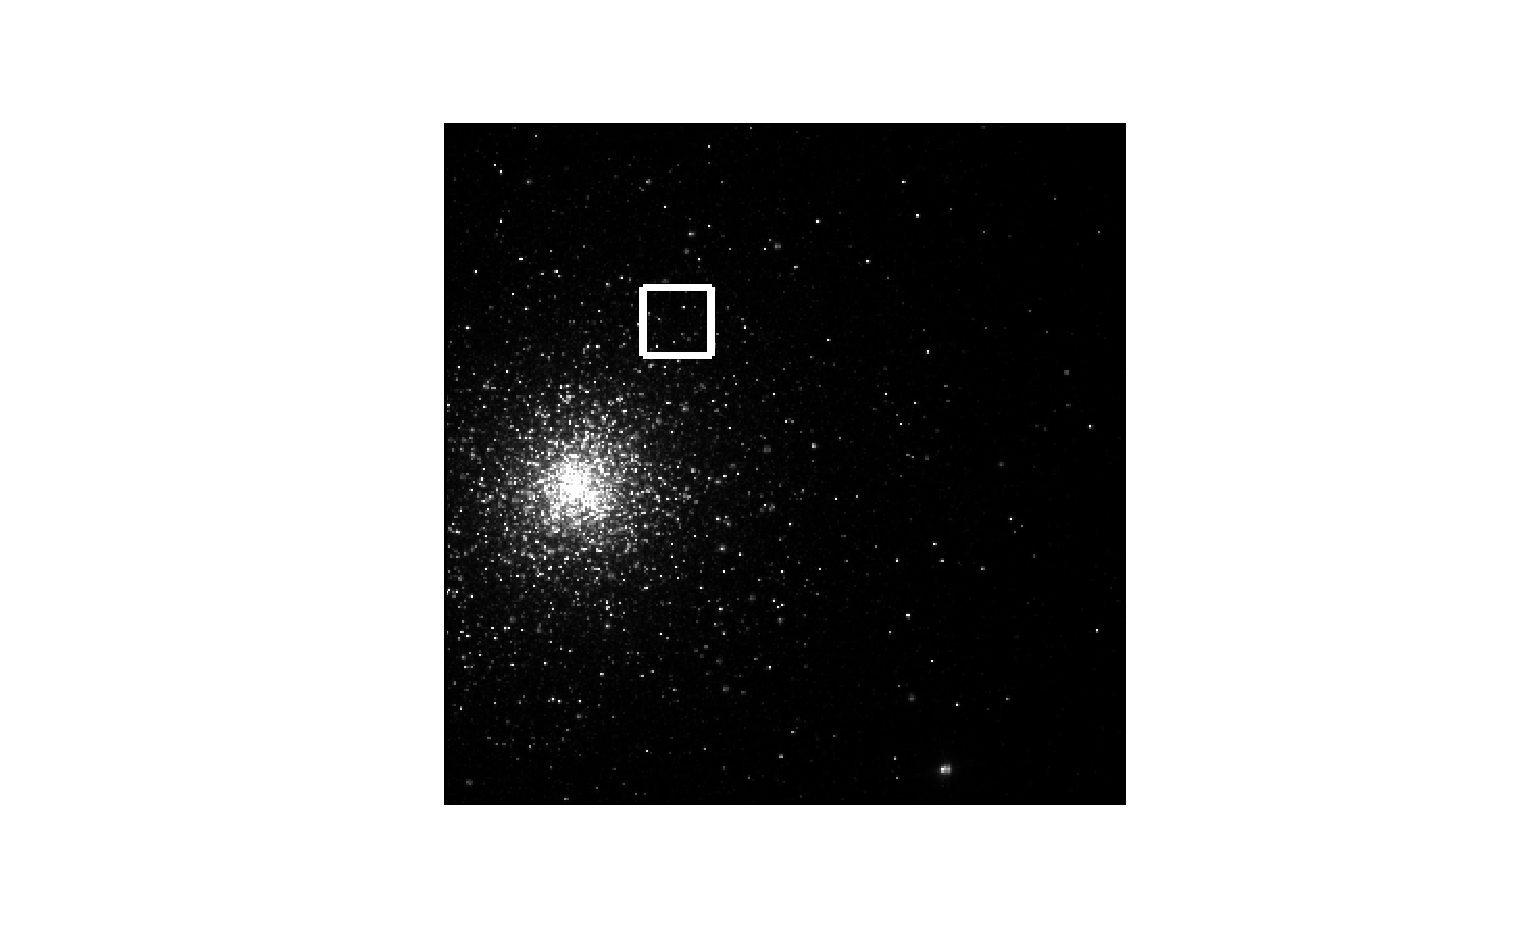
\includegraphics[width=0.7\textwidth]{figures_vg/m2_results/m2_regions.eps}
%    \vspace{-1cm}
    \caption{The M2 globular cluster as imaged by SDSS. In white is $100 \times 100$ subregion 
    cataloged by PCAT in \cite{Feder_2019}. }
    \label{fig:m2_region}
\end{figure}

The M2 globular cluster is a crowded starfield found in field 136 of camera column 2 in run 2583 of the SDSS survey. 
M2 was also imaged in the ACS Globular Cluster Survey~\citep{Sarajedini_2007}
using the Hubble Space Telescope (HST),
which has greater resolution than the SDSS telescope.
The resolution of the HST wide-field channel is 0.05 arcseconds per pixel versus
0.40 arcseconds per pixel in SDSS \citep{hubble_about, sdss_about}.
For this image, the catalog from the HST survey (henceforth the ``HST catalog")
serves as ground truth for validating our results.

We first analyze the $100 \times 100$ pixel subimage of M2 that
\cite{Portillo_2017} and \cite{Feder_2019} analyzed with their MCMC-based approach, PCAT.
This subimage shows a region located outside the heavily saturated core of the cluster (Figure~\ref{fig:m2_region}). 
Nonetheless, in this subimage the HST catalog contains 1114 stars with F606W-band magnitudes less than 22.
We include two bands in our model, the SDSS $r$-band and $i$-band.
The SDSS $r$-band and the Hubble F606W band are centered at roughly the same wavelength,
while the wavelength range of the Hubble F606W band is slightly broader.

We compare the cataloging accuracy of StarNet
against PCAT, the aforementioned MCMC-based approach that uses the same generative model as StarNet;
and DAOPHOT, an algorithmic routine for detecting stars in crowded starfields
which does not use a probabilistic model~\citep{stetson2987daophot}.
DAOPHOT convolves the observed image with a Gaussian kernel and scans for peaks above a given threshold.
The DAOPHOT catalog of M2 was reported in \cite{An_2008_m2}.


% Both DAOPHOT and the Hubble survey produce a single catalog -- that is, a set of estimated stellar locations and fluxes -- with
% error bars nominally representing marginal uncertainties.
% In the context of probabilistic cataloging (StarNet and PCAT), the posterior
% defines a distribution over catalogs.
% Each sample from the (approximate) posterior returns a catalog, and each
% sampled catalog may have different cardinally.

To evaluate the three methods, we filtered the ground truth HST catalog to stars with magnitudes smaller than 22.5 in the Hubble F606W band
(note that smaller magnitude corresponds to brighter stars),
because none of the three methods were able to detect stars
with lower apparent brightness in the SDSS image.


Estimated catalogs are evaluated on three metrics: the true positive rate (TPR), or recall;
the positive predictive value (PPV), or precision;
and the F1 score.
The TPR is the proportion of true stars in the HST catalog matched with a predicted star in the estimated catalog.
The PPV is the proportion of predicted stars in the estimated catalog matched with a true star in the HST catalog.
The F1 score summarizes the two metrics as the harmonic mean of the PPV and the TPR.

Like \cite{Portillo_2017} and \cite{Feder_2019}, we define a ``match" between an estimated star
and an HST star as follows: (1) the estimated location and the HST location are within 0.5 SDSS pixels,
and (2) the estimated SDSS $r$-band flux and the HST F606W band flux are within half a magnitude.
% The slack in magnitude accounts for the fact that the wavelength range of the HST F606W band is slightly broader than the SDSS $r$-band (though they are centered at roughly the same wavelength).

In probabilistic cataloging (PCAT and StarNet), the posterior defines a distribution over catalogs.
For StarNet, the TPR, PPV, and F1 score were computed for the catalog corresponding to the mode of the variational distribution (henceforth, the StarNet catalog).
For PCAT, 300 catalogs were sampled using MCMC; the metrics were computed for each sampled catalog and averaged.

\begin{figure}[tb]
    \centering
    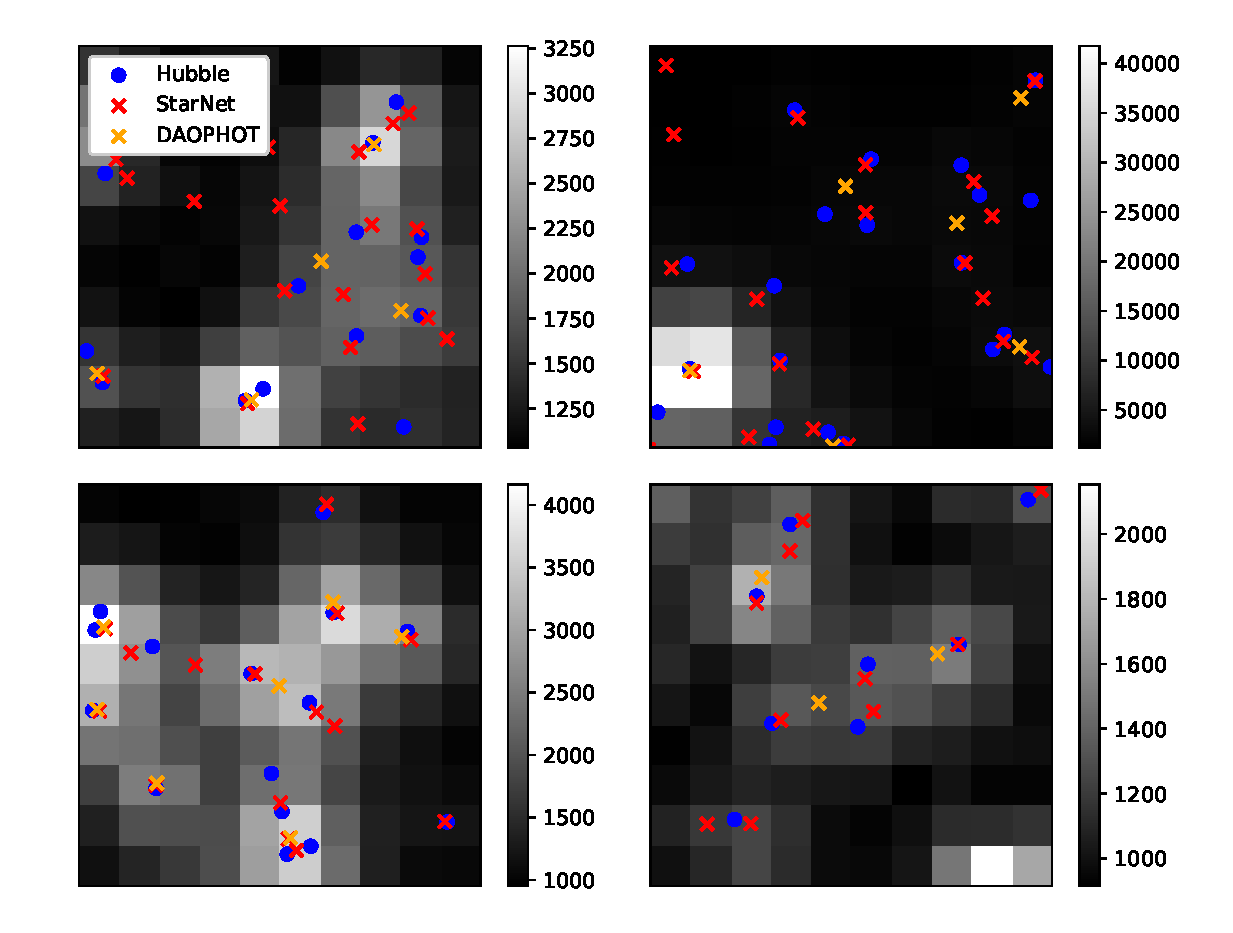
\includegraphics[width=0.49\textwidth]{figures_vg/m2_results/example_subimages_starnet.eps}
    \rulesep
    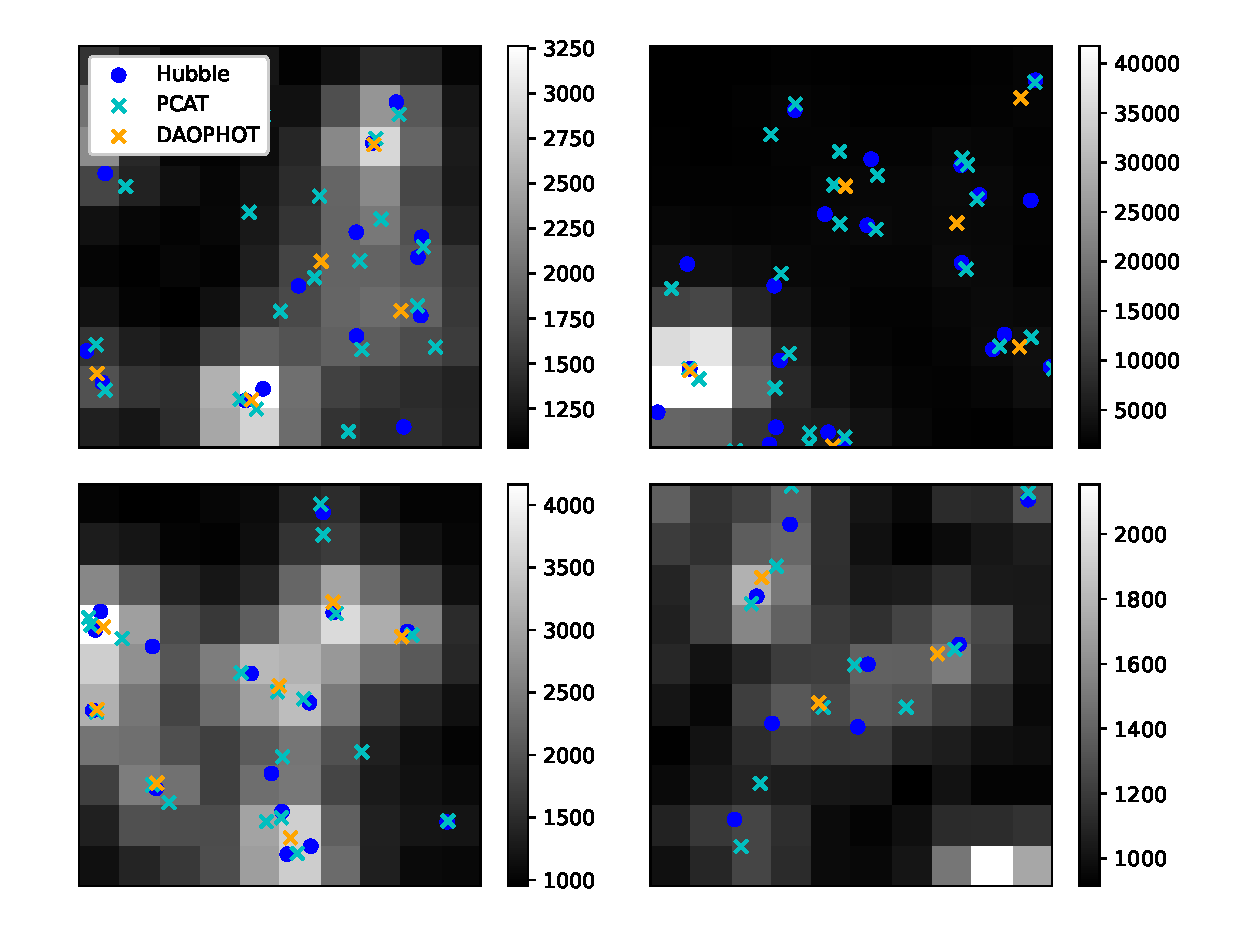
\includegraphics[width=0.49\textwidth]{figures_vg/m2_results/example_subimages_pcat.eps}
    % \vspace{-1cm}
    \caption{Estimated catalogs on four 10$\times$10 subimages from
    M2. Blue dots are stars from the HST catalog used as ground truth.
    StarNet, PCAT, and DAOPHOT estimated stars are shown as
    red, cyan, and orange crosses, respectively. }
    \label{fig:example_subimages}
\end{figure}

StarNet produced a catalog that outperforms DAOPHOT and PCAT in F1 score (Table~\ref{tab:summary_stats}).
Figure~\ref{fig:example_subimages} compares the StarNet catalog to the PCAT, DAOPHOT, and HST catalogs.
DAOPHOT estimated less than half the number of stars when compared to the other methods.
It therefore had a large PPV but a small TPR.
The StarNet catalog had similar TPR as PCAT while having an 11\% higher PPV.

The improvement of StarNet over PCAT in PPV was most pronounced for the brightest stars (Figure~\ref{fig:summary_stats}), 
suggesting that the brightest stars in the PCAT catalog may have in truth been a collection of blended dim stars. 
The TPR for StarNet was uniformly better than DAOPHOT across all magnitudes.
Of all methods, StarNet best approximated the HST flux distribution (Figure~\ref{fig:luminosity_fun_m2}).

Table~\ref{tab:summary_stats} also shows the number of stars inferred by each method.
There are 1114 stars in the HST catalog.
For probabilistic methods (StarNet and PCAT),
we display the mean number of stars under the approximate posterior, along with the 5th and 95th percentiles.
We compute the StarNet posterior mean and quantiles by sampling from the variational posterior. 
Recall that on each tile, the variational posterior on the number of stars is a categorical random variable; 
to construct a distribution for the number of stars on the whole image, we first sample from the per-tile categorical distribution, then sum over all tiles. 
StarNet posterior intervals were three times wider than the PCAT intervals.
The small PCAT intervals may indicate that the MCMC sampler failed to mix well. 
However, both StarNet and PCAT intervals fail to cover the ground truth. 
We attribute the over-estimated number of stars by StarNet to the tiling structure of 
the approximate posterior (Appendix~\ref{sec:coverage}). 

% \begin{table}[!tb]
% \centering
% \caption{Performance metrics on M2.
% For probabilistic methods (StarNet and PCAT)
% the ``\#stars" column refers to the mean number of stars under the (approximate) posterior, while the right-most column displays the 5-th and 95-th percentiles under the posterior. }
% \label{tab:summary_stats}
% \begin{tabular}{l|ccc|cc}
% \toprule
%      Method &   TPR &   PPV &  F1 score &  \#stars & (q-5\%, q-95\%)\\
% \midrule
%     DAOPHOT &  0.20 &  0.63 &      0.30 &     295 & -- \\
%        PCAT &  0.56 &  0.40 &      0.47 &    1672 & (1664, 1680)\\
%  Sleep-only &  0.51 &  0.47 &      0.49 &    1292 & (1260, 1324)\\
%  Wake-sleep &  0.51 &  0.60 &      0.55 &     1014 & (987, 1041)\\
%      %Hubble &  1.00 &  1.00 &      1.00 &     1114 & -- %\\
% \bottomrule
% \end{tabular}
% \end{table}

\begin{table}[!tb]
\centering
\caption{Performance metrics on M2.
For probabilistic methods (StarNet and PCAT)
the ``\#stars" columns provide the mean along with the 5th and 95th percentiles
for the number of stars under the (approximate) posterior,
The number of stars in the Hubble catalog is 1114. }
\label{tab:summary_stats}
\begin{tabular}{l|ccc|cc}
\toprule
& & & & \multicolumn{2}{c}{\#Stars} \\
     Method &   TPR &   PPV &  F1 score &  mean & (q-5\%, q-95\%)\\
\midrule
    DAOPHOT &  0.20 &  0.65 &      0.31 &     357 & -- \\
       PCAT &  0.55 &  0.37 &      0.44 &    1672 & (1664, 1680)\\
 StarNet (our) &  0.53 &  0.48 &      \textbf{0.50} &    1462 & (1430, 1497)\\
\bottomrule
\end{tabular}
\end{table}


% PCAT overestimated the number of dim stars with magnitudes greater than 21.
% In contrast, DAOPHOT failed to find stars with magnitudes greater than $21$.

% (Figures~\ref{fig:m2_flux_estimation} and \ref{fig:luminosity_fun_m2}).

\begin{figure}[tb]
    \centering
    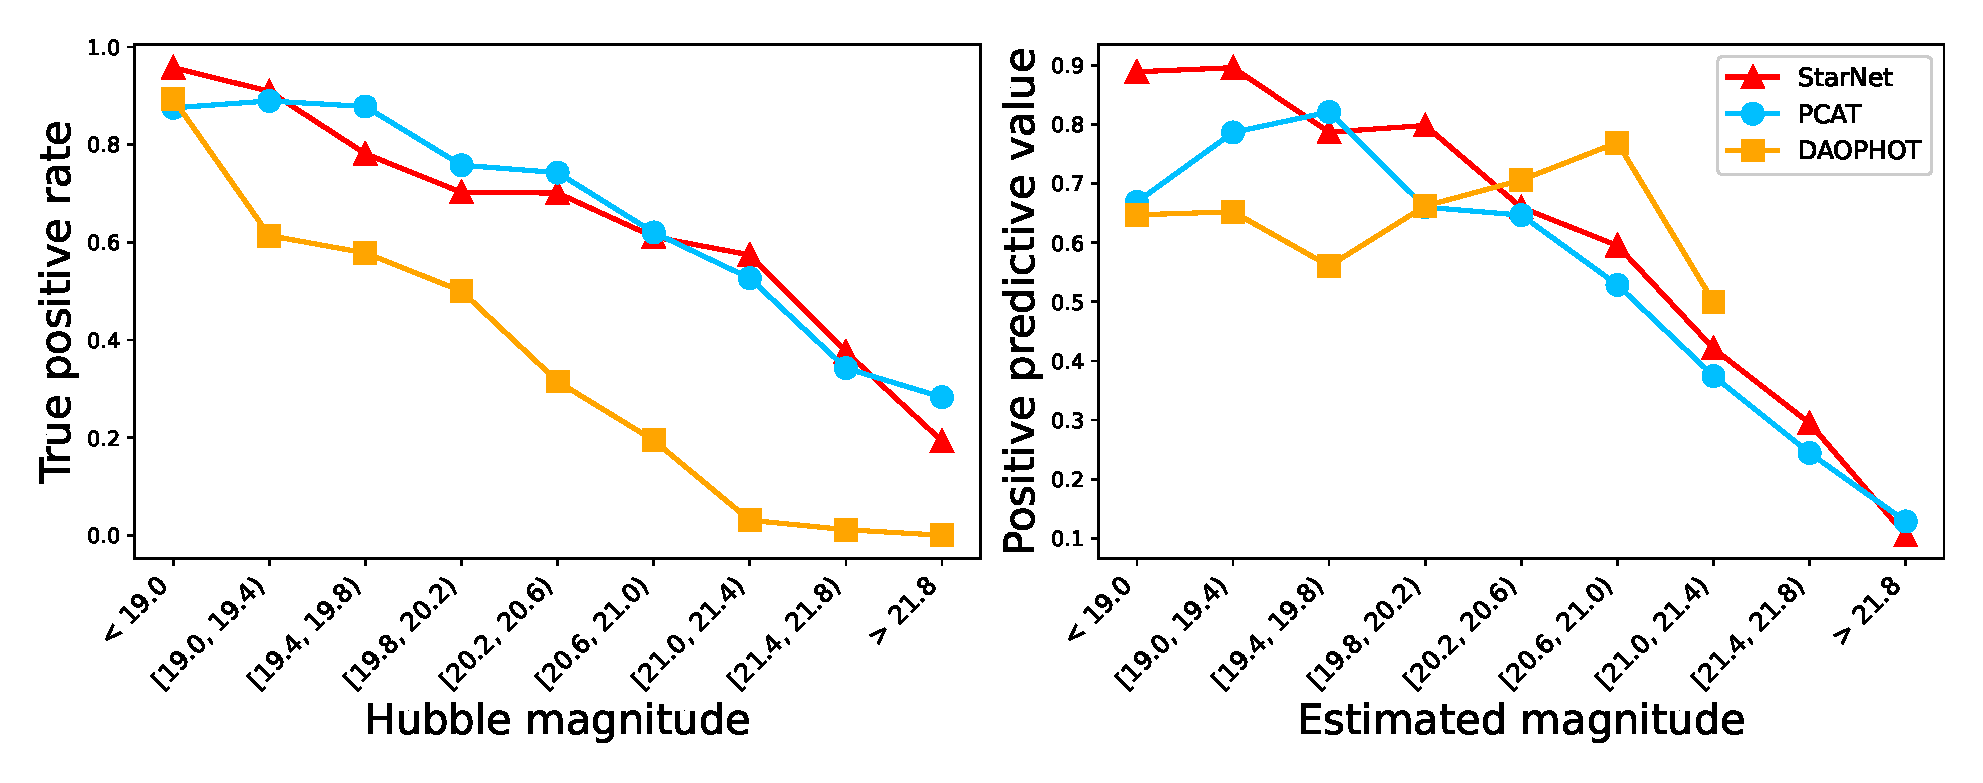
\includegraphics[width=0.99\textwidth]{figures_vg/m2_results/summary_statistics_m2.eps}
%    \vspace{-0.4cm}
    \caption{True positive rate (left) and positive predicted value (right) of various cataloging
    procedures on M2, plotted against $r$-band magnitude.
    Smaller magnitudes correspond to brighter stars.
    }
    \label{fig:summary_stats}
\end{figure}

% \begin{figure}[tb]
%     \centering
%     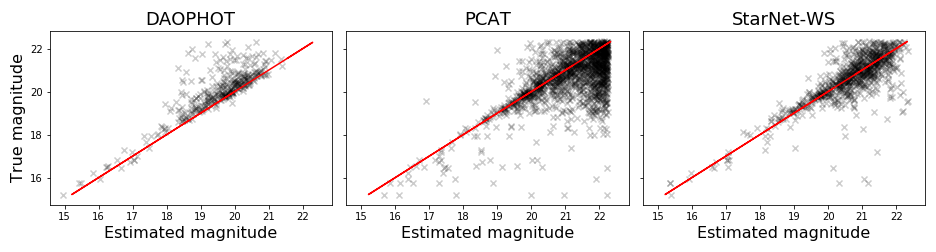
\includegraphics[width=0.99\textwidth]{figures/m2_results/m2_flux_estimation.png}
%     \caption{True versus estimated magnitudes on the $r$-band of M2.
%     Every estimated star was matched with the nearest Hubble star in L2 distance between locations.
%     Red line is the identity, $y=x$. }
%     \label{fig:m2_flux_estimation}
% \end{figure}

\begin{figure}[tb]
    \centering
    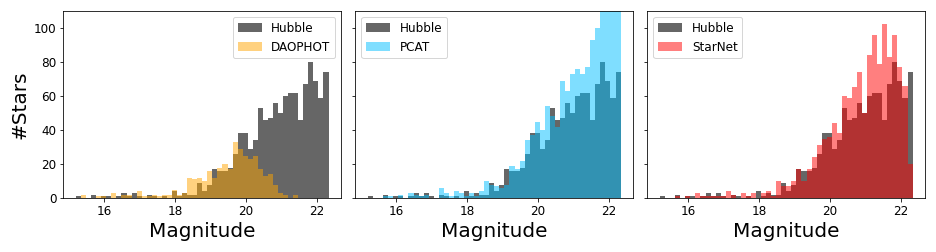
\includegraphics[width=0.99\textwidth]{figures/m2_results/luminosity_fun.png}
%    \vspace{-0.4cm}
    \caption{Flux distributions for the $r$-band observations of M2.
    The flux distribution of the HST catalog is in grey.
    Estimated distributions from DAOPHOT, PCAT, and StarNet catalogs are overlaid.
    For PCAT, the flux distribution is from a single catalog sample. }
    \label{fig:luminosity_fun_m2}
\end{figure}


% \begin{figure}[tb]
%     \centering
%     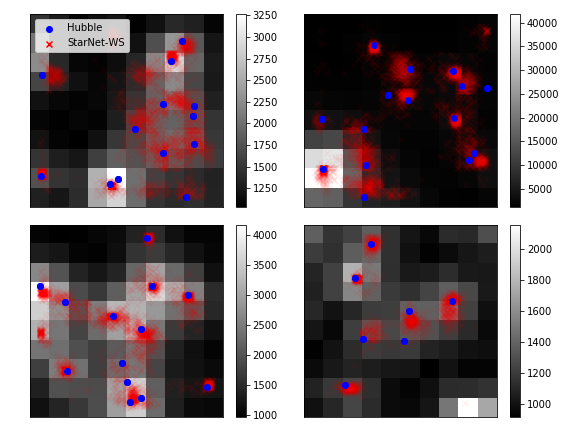
\includegraphics[width=0.49\textwidth]{figures/m2_results/example_subimages_samples_ws.png}
%     \rulesep
%     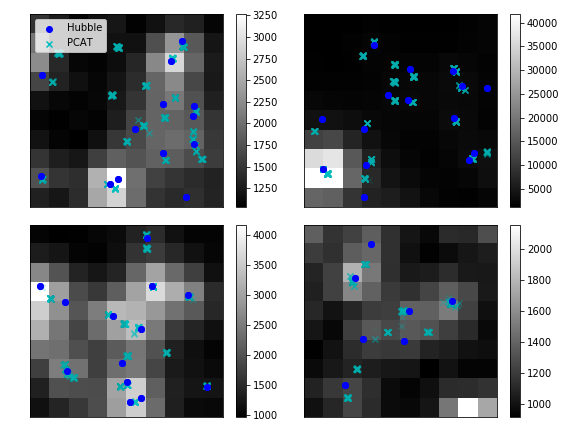
\includegraphics[width=0.49\textwidth]{figures/m2_results/example_subimages_samples_pcat.png}
%     \caption{Four 10$\times$10 subimages from
%     M2. Blue dots are stars from the HST catalog used as ground truth. (Left) Posterior samples from StarNet-WS and (right) posterior samples from the MCMC chain of PCAT. }
%     \label{fig:example_subimages_sampled}
% \end{figure}

% StarNet-WS returns a well-defined distribution over the set of all catalogs
% and is thus able to capture uncertainties in catalog construction.
% Samples from the StarNet-WS variational distribution are compared with samples from PCAT in Figure~\ref{fig:example_subimages_sampled}.

In a subsequent experiment, 
we go beyond the $100\times100$ subimage
cataloged by \cite{Feder_2019} and 
catalog the entire M2 globular cluster 
contained in a $1000 \times 1000$-pixel image (Figure~\ref{fig:m2_region}). 
We produce a color-magnitude diagram on this entire region (Figure~\ref{fig:m2_cmd}). 
On the entire region, a second distinct cluster, 
shifted to the right in color, 
appears in addition to the main sequence of stars.
The second cluster becomes more apparent after we filter to high-confidence stars in the StarNet catalog, 
defined as stars with flux posterior standard deviation less than one. 
This second cluster, corresponding to a collection of red giants, 
is undetectable without the ability of StarNet to 
scale to larger images. 

However, 
the patterns are less definite in the StarNet color-magnitude diagram than in the Hubble color magnitude diagram.
There is more spread in the StarNet color estimates, particularly at faint magnitudes. 
This is due to the superior resolution of the Hubble telescope; near the heavily saturated core of the M2 cluster, stars are near impossible to deblend in the SDSS image, and our performance suffers (Appendix~\ref{sec:test_m2}). 


% Most of the cataloged stars lie on the 
% main sequence of stars, but
% we also see a second cluster of stars 
% with a shift in color. These correspond to 
% a collection of red giants. 


\begin{figure}[tb]
    \centering
    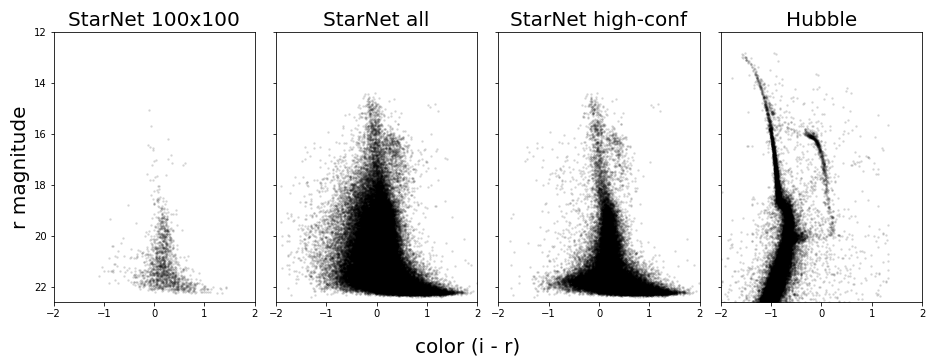
\includegraphics[width=0.99\textwidth]{figures/m2_results/m2_cmd.png}
%    \vspace{-0.5cm}
    \caption{Color-magnitude diagrams from StarNet and Hubble. From left to right, color-magnitude diagrams constructed from: the same $100\times100$ subimage as was cataloged in \cite{Feder_2019}; 
    the StarNet catalog derived from the entire $1000 \times 1000$ image of M2; 
    that StarNet catalog, filtered to stars with posterior SD(flux) $< 1$; the Hubble catalog. 
}
    \label{fig:m2_cmd}
\end{figure}


% Figure~\ref{fig:cmd_m2} displays the estimated color-magnitude diagrams. While the Hubble F606W-band corresponds roughly to the SDSS $r$-band, there is no such correspondence for the SDSS $i$-band. Thus, using the Hubble locations, we estimated the $i$-band fluxes using maximum likelihood: letting $x^{(i)}$ be the SDSS image in the $i$-band, $N_H$ the number of stars in the Hubble catalog and $\ell_H$ their locations, solve
% \begin{align}
%   f^{(i)}_H = \argmax_{f\in\mathbb{R}^{N_H}} \log p(x^{(i)} | N_H, \ell_H, f)
%   \label{eq:optim_iband_flux},
% \end{align}
% where the log likelihood is given by the generative model from Section~\ref{sec:gen_model}.
% The estimated $i$-band fluxes and the reported Hubble F606W-band fluxes $f_H^{(r)}$ define the ``true" colors, $2.5\log(f_H^{(i)}/f_H^{(r)})$.
% In the color magnitude diagram, DAOPHOT did not capture the full spectrum of colors; of all three methods, PCAT best captured the color spectrum. All three methods however, were able to capture the arm thing (TODO there is a name for this ... main sequence turnoff?) that branches off at low magnitudes.

% \begin{figure}[ht]
%     \centering
%     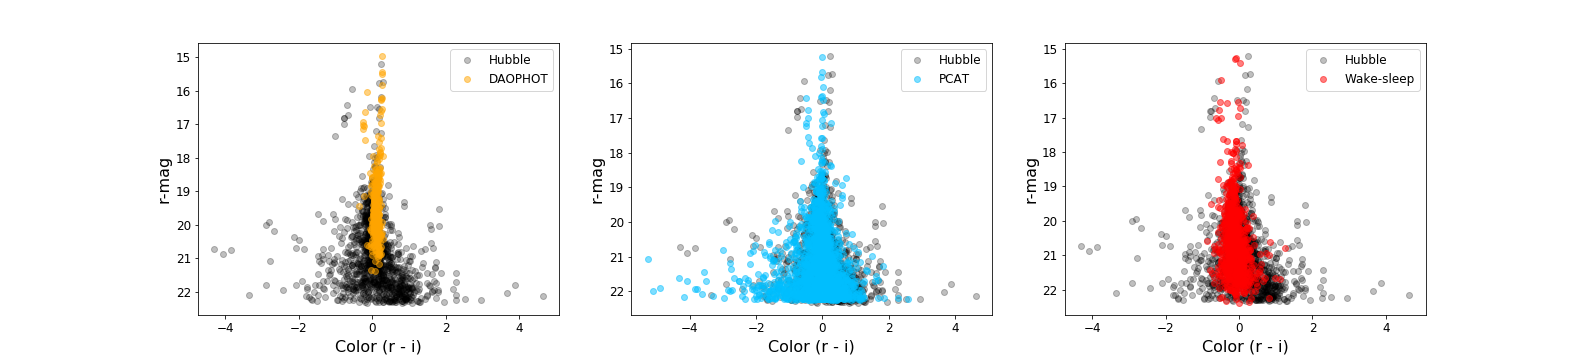
\includegraphics[width=0.99\textwidth]{figures/cmd.png}
%     \caption{Color magnitude diagrams on M2. }
%     \label{fig:cmd_m2}
% \end{figure}



% Figure~\ref{fig:loglik_table} displays the log-likelihood under the default SDSS estimates of the PSF and background compared with the estimates found using wake-sleep.
% The wake-sleep estimates improved the log-likelihood.
% We also compared against the ``Hubble estimate" of the background and PSF, obtained by minimizing $- \log p_\phi(x | N_{H}, \ell_{H}, f_{H})$ for $\phi$ directly.

% The results suggest that the primary source of model misfit is the background. A significant increase in log-likelihood occurred by switching from the SDSS background to the Hubble-estimated background.
% But even using the Hubble-estimated background, switching from the SDSS PSF to our wake-sleep PSF improves the log-likelihood.

% \begin{figure}[ht]
%     \centering
%     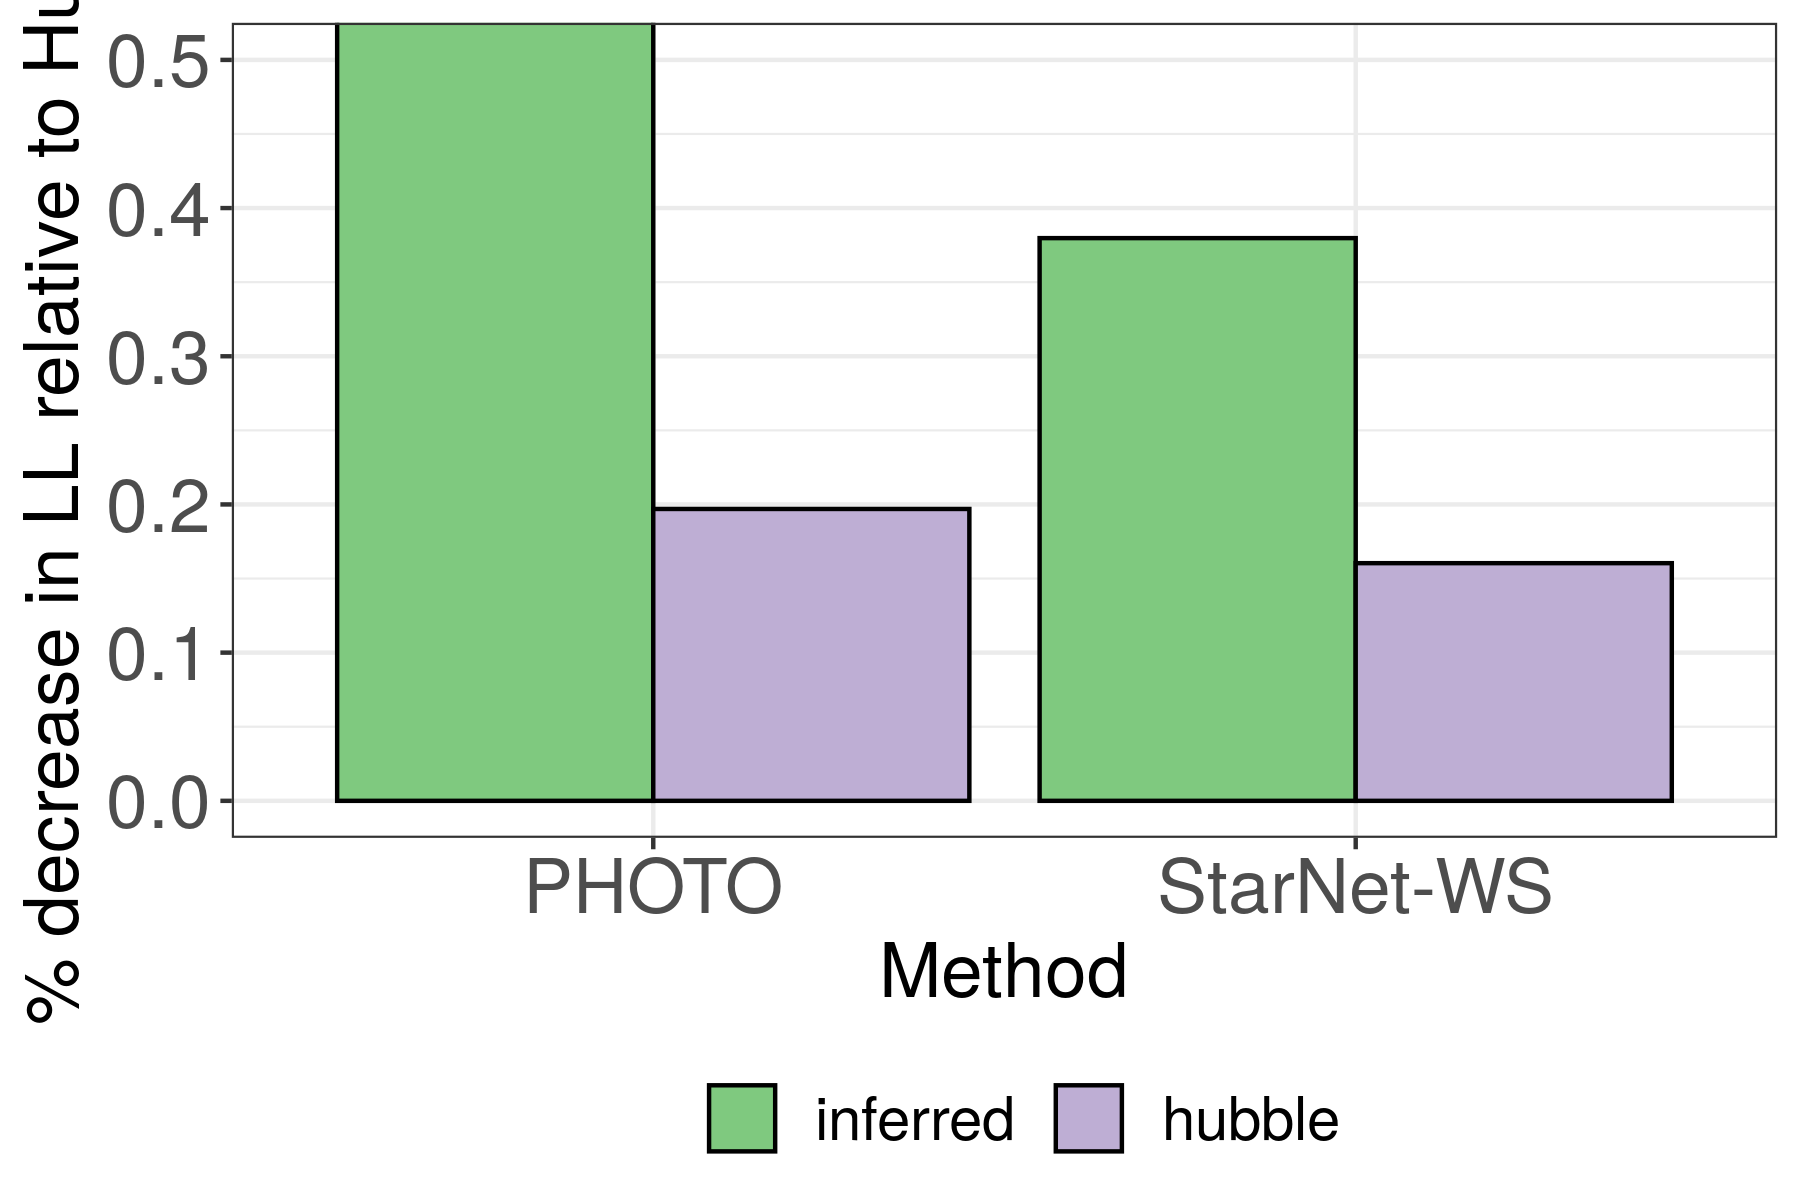
\includegraphics[width=0.6\textwidth]{figures/loglik_table.png}
%     \caption{Percent decrease in log-likelihood relative to the Hubble estimate of the PSF and background.
%     For each method, we evaluate the log-likelihood where the both PSF
%     and background are estimated (green);
%     we also show results where only the PSF is estimated (purple).
%     }
%     \label{fig:loglik_table}
% \end{figure}

% \input{tables/chi_sq_stats.txt}
% \caption{
% Negative log-likelihood for SDSS, wake-sleep, and Hubble estimated model parameters. In the right column, we fix the background to the Hubble estimate, and examine negative log-likelihood as the PSF varies.}

% The StarNet-based PSF did not differ from the SDSS PSF significantly. The greatest change was in the $r$-band PSF, where the SDSS PSF was most different from the Hubble-estimated PSF.

% \begin{figure}[ht]
%     \centering
%     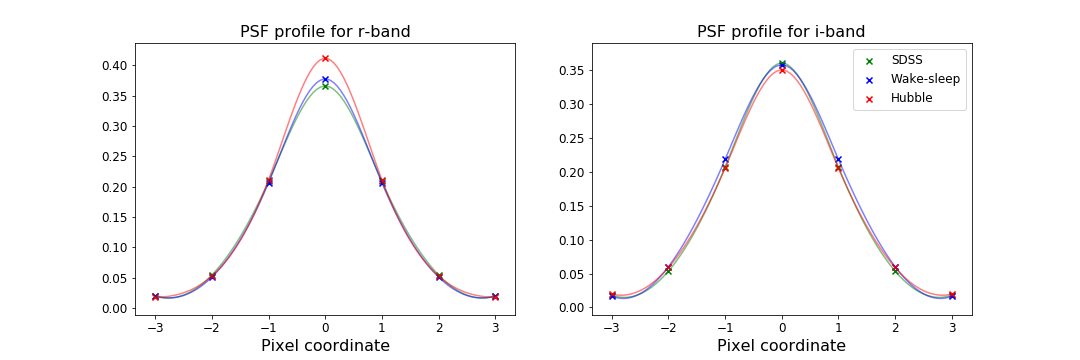
\includegraphics[width=0.99\textwidth]{figures/psf_profiles.png}
%     \caption{Estimated versus true PSF profiles on M2. The Hubble PSF was
%     obtained by optimizing the likelihood conditioned on locations and fluxes
%     from the Hubble catalog. TODO: this image is not that informative, I think I'll remove this. }
%     \label{fig:psf_profiles}
% \end{figure}


% \multicolumn{1}{p{5cm}}{\raggedleft Neg. loglik \\ (with Hubble back.)}
% \caption{
% Chi-squared statistics for SDSS, wake-sleep, and Hubble estimated model parameters.
% The chi-squared statistic is defined as
% $\sum_{bij}\frac{([\text{obs.image}]_{bij} - [\text{recon.image}]_{bij})^2}{[\text{recon.image}]_{bij}}$.
% In the middle column, ``model parameters" refer to both background and PSF.
% In the right column, we fix the background to the Hubble estimate, and examine
% chi-squared statistics as the PSF varies.}
